\documentclass[aspectratio=169]{beamer}
\usepackage[T1]{fontenc}
\usepackage[utf8]{inputenc}
\usepackage{tikz}
\usepackage{tabularx}
\usepackage[font=scriptsize]{caption}
\captionsetup[figure]{labelformat=empty}

\usetikzlibrary{tikzmark,shapes,arrows,backgrounds,fit,positioning}
\newcolumntype{C}{>{\centering\arraybackslash}X}
\newcolumntype{R}{>{\raggedleft\arraybackslash}X}

\addtobeamertemplate{navigation symbols}{}
{
	\insertframenumber{}
}

\beamertemplatenavigationsymbolsempty
\setbeamercolor{section in foot}{fg=white, bg=blue}
\setbeamercolor{subsection in foot}{fg=black, bg=white}
\setbeamerfont{footline}{size=\fontsize{6}{6}\selectfont}

\setbeamertemplate{footline}
{
  \leavevmode
  \hbox
  {
    \begin{beamercolorbox}
      [wd=.5\paperwidth,ht=2.5ex,dp=1.125ex,leftskip=.3cm,rightskip=.3cm]{subsection in foot}
    \end{beamercolorbox}
    
    \begin{beamercolorbox}
      [wd=.5\paperwidth,ht=2.5ex,dp=1.125ex,leftskip=.3cm,rightskip=.3cm plus1fil]{subsection in foot}
      \hfill
      \insertframenumber
      %\insertframenumber\,/\,\inserttotalframenumber
    \end{beamercolorbox}
  }
}



\title{UUB Charge and Peak histograms}
\author{
  Mauricio Su\'arez Dur\'an and Ioana~C.~Mari\c{s}
}
\institute{IIHE-ULB}

\titlegraphic{
  \begin{figure}[h]
    \centering
   %
\includegraphics[width=5cm]{ulbLogo2.png}
    \hspace*{8.cm}
    
\includegraphics[width=5.5cm]{iihe.jpeg}
  \end{figure}
}

\begin{document}
\begin{frame}
  \titlepage
\end{frame}


\begin{frame}
	\frametitle{UUB Charge and Peak histograms}
	\begin{itemize}
		\item Station studied: 863 1222 1219 1211 1740 1743 1221 1223 1217 1747 1741 1745 1818 1851 1729 1735 1746 1819 1791
		\item Data from CDAS.
		\item {\underline {Software CDAS, pre-production version.}}
	\end{itemize}
	\centering
	\includegraphics[width=.45\textwidth]{mapStations.pdf}
\end{frame}


\begin{frame}
  \frametitle{A/P}
  \begin{figure}
    \centering
    \begin{tabularx}{\textwidth}{CC}
      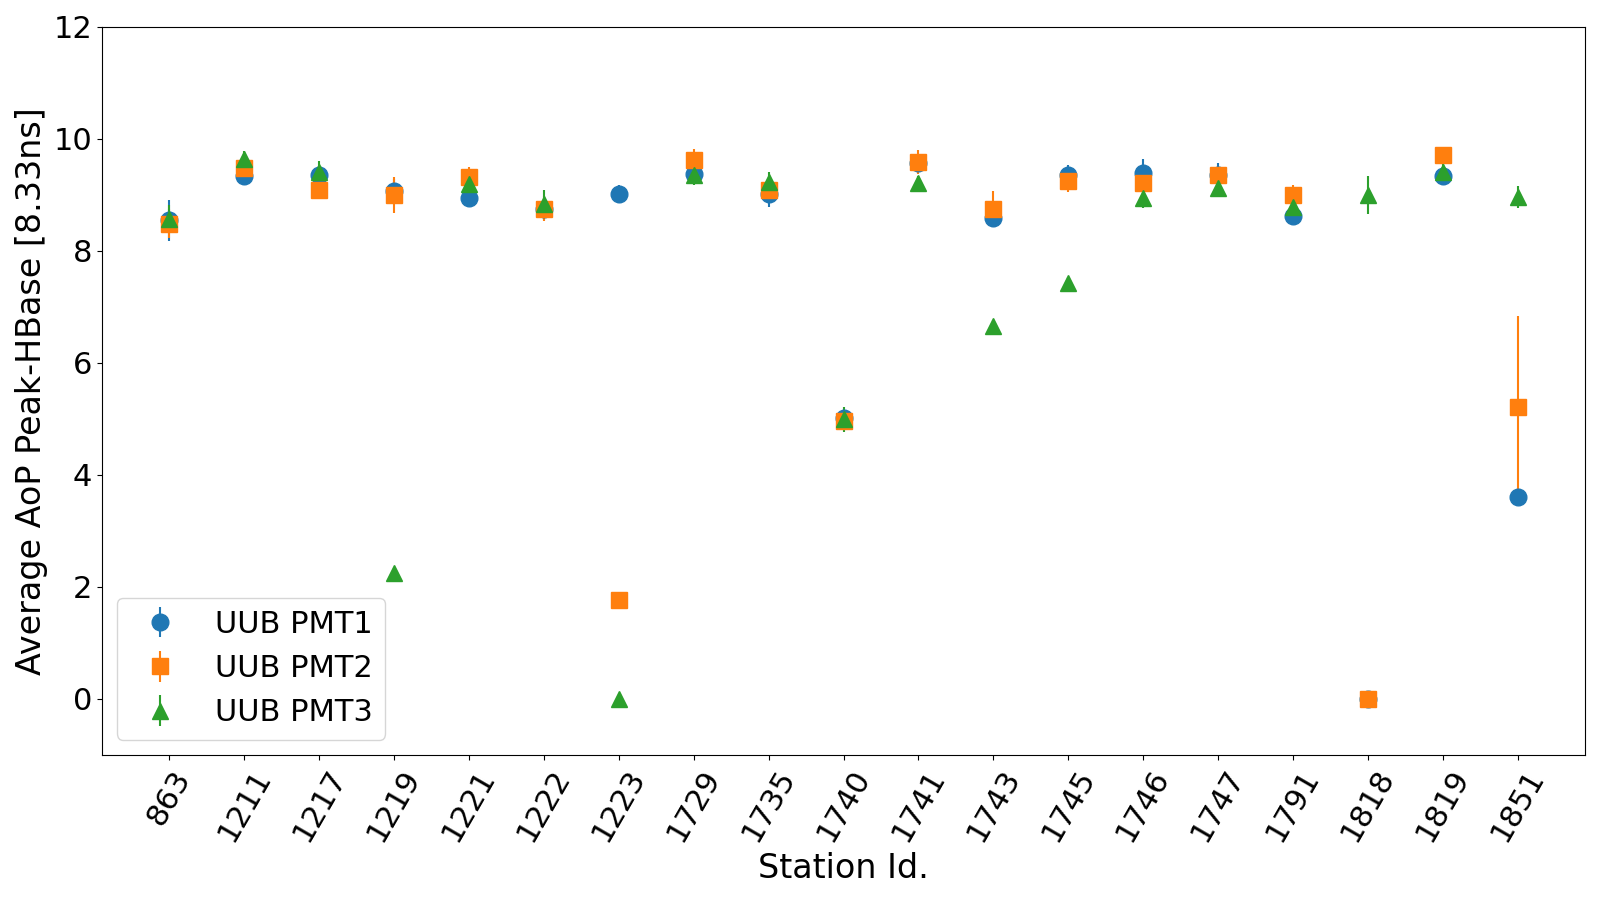
\includegraphics[width=.45\textwidth]{../plots/uubAoPHbasePMTs.png}
      &
      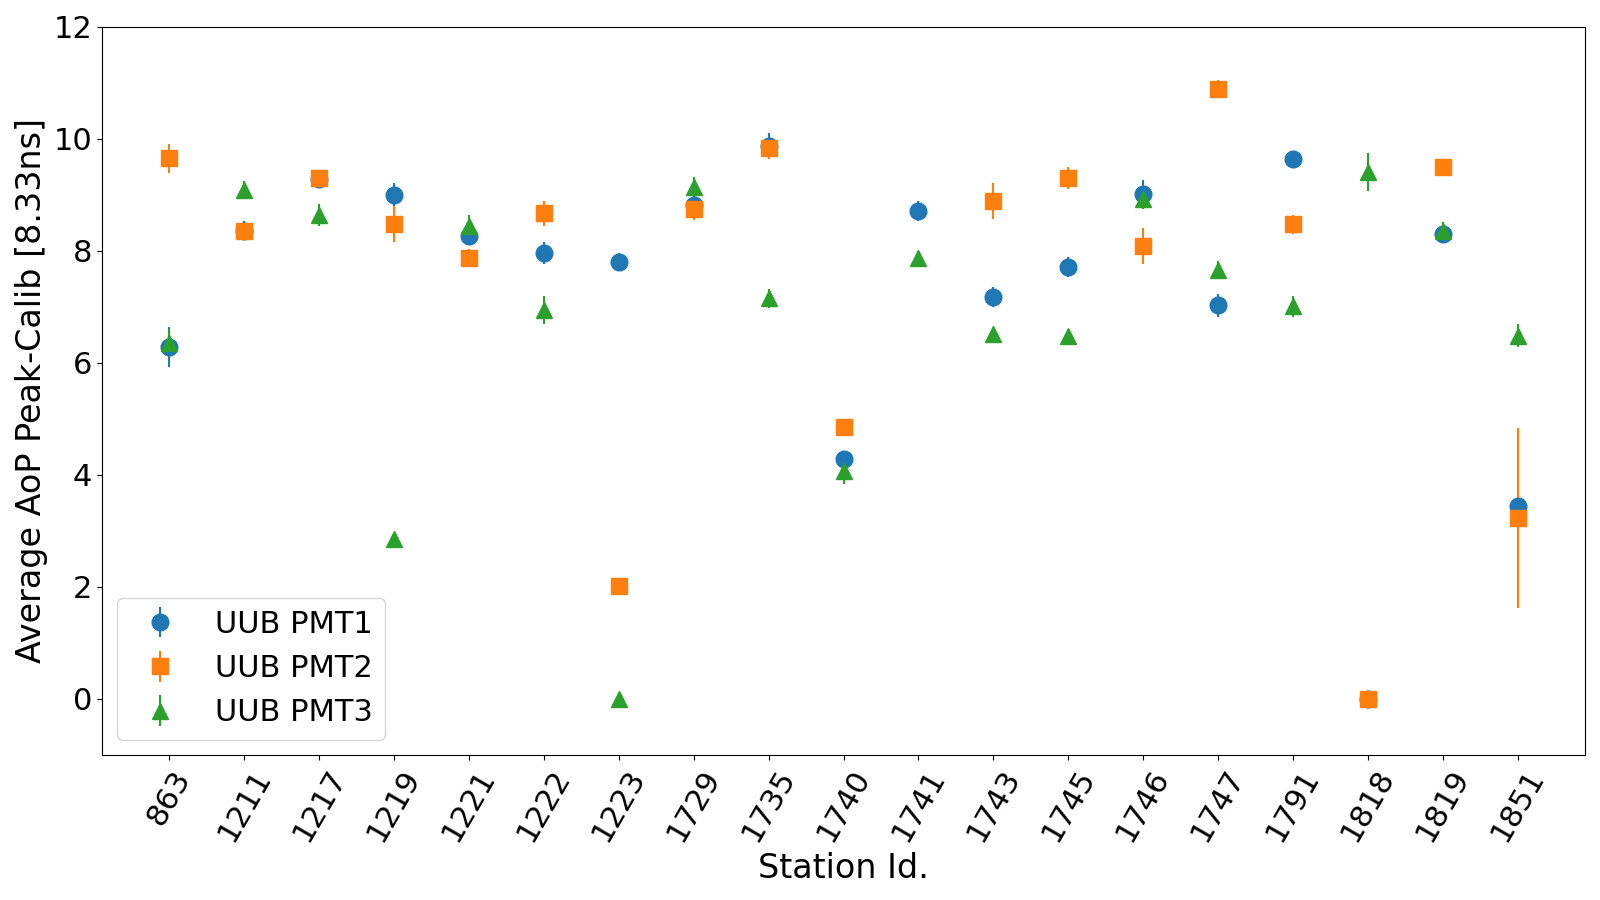
\includegraphics[width=.45\textwidth]{../plots/uubAoPCalibPMTs.png}
      \\
      \includegraphics[width=.45\textwidth]{../plots/ubAoPHbasePMTs.png}
      &
      \includegraphics[width=.45\textwidth]{../plots/ubAoPCalibPMTs.png}
    \end{tabularx}
  \end{figure}
  \centering
  
\end{frame}


\begin{frame}
  \frametitle{A/P Relative difference for Peak corrections}
  \begin{figure}
    PMTs with AoP lower than $4$\,ns for UUB and $2$\,ns for UB are not considered here.
    \centering
    \begin{tabularx}{\textwidth}{CC}
      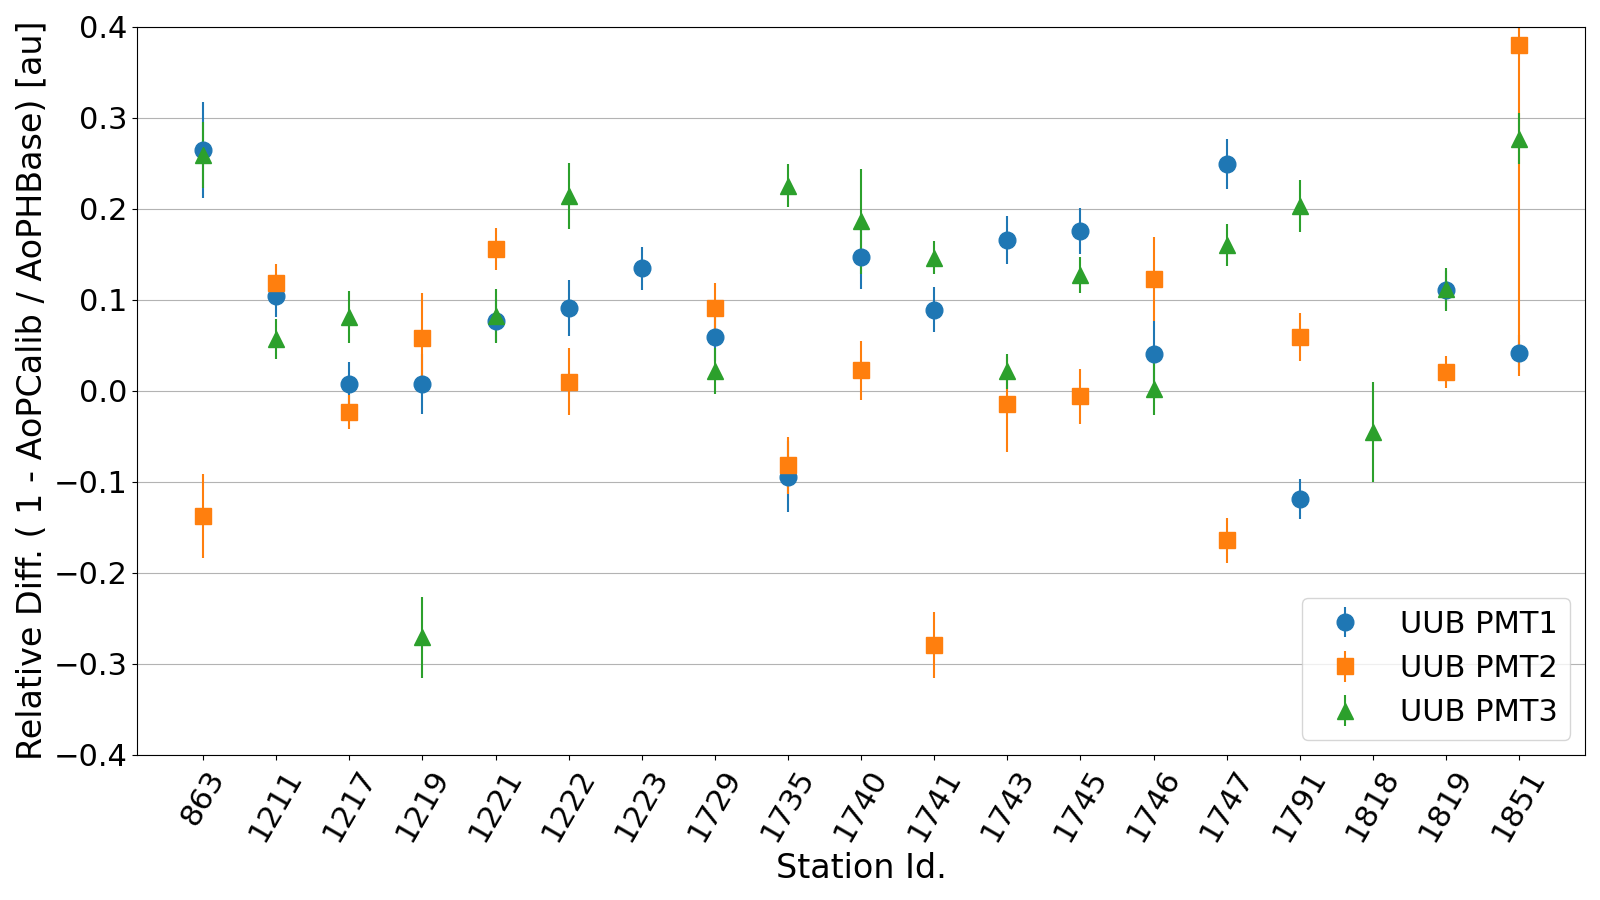
\includegraphics[width=.43\textwidth]{../plots/uubAoPDiffCaHbPMTs.png}
      &
      \includegraphics[width=.43\textwidth]{../plots/ubAoPDiffCaHbPMTs.png}
      \\
      \includegraphics[width=.43\textwidth]{../plots/aopHbaseUubUbPMTs.png}
      &
      \includegraphics[width=.43\textwidth]{../plots/aoCalibUubUbPMTs.png}
    \end{tabularx}
  \end{figure}
\end{frame}


\begin{frame}
	\frametitle{Peak and Charge over time}
  \begin{figure}
  \centering
    \begin{tabularx}{\textwidth}{CC}
      \includegraphics[width=.5\textwidth]{../plots/uubPeaktimeHbSt863PMTs.png}
      &
      \includegraphics[width=.5\textwidth]{../plots/uububChargetimeHbSt863PMTs.png}
    \end{tabularx}
  \end{figure}
\end{frame}

\begin{frame}
	\frametitle{Peak and Charge over time}
  \begin{figure}
  \centering
    \begin{tabularx}{\textwidth}{CC}
      \includegraphics[width=.5\textwidth]{../plots/uubPeaktimeHbSt1740PMTs.png}
      &
      \includegraphics[width=.5\textwidth]{../plots/uububChargetimeHbSt1740PMTs.png}
    \end{tabularx}
  \end{figure}
\end{frame}


\begin{frame}
	\frametitle{Peak and Charge over time}
  \begin{figure}
  \centering
    \begin{tabularx}{\textwidth}{CC}
      \includegraphics[width=.5\textwidth]{../plots/uubPeaktimeHbSt1219PMTs.png}
      &
      \includegraphics[width=.5\textwidth]{../plots/uububChargetimeHbSt1219PMTs.png}
    \end{tabularx}
  \end{figure}
\end{frame}


\begin{frame}
  \frametitle{How well is the fit method works? }
  {\bf Events-Fitting / Events-total }
	\begin{figure}
		\centering
    \begin{tabularx}{\textwidth}{CC}
      \begin{tabular}{l}
        \includegraphics[width=.44\textwidth]{../plots/uubGoodFitEvtnPk.png}
      \end{tabular}
      &
			\begin{tabular}{l}
				\includegraphics[width=.44\textwidth]{../plots/ubGoodFitEvtnPk.png}
			\end{tabular}
			\\
			\begin{tabular}{l}
				\includegraphics[width=.44\textwidth]{../plots/uubGoodFitEvtnChPMT.png}
			\end{tabular} 
      &
      \begin{tabular}{l}
        \includegraphics[width=.44\textwidth]{../plots/ubGoodFitEvtnChPMT.png}
      \end{tabular}
		\end{tabularx}
	\end{figure}
\end{frame}



\end{document}
